\documentclass[../main.tex]{subfiles}

\begin{document}
Emotions play a massive role in our everyday life. 
They affect how we react to certain situations. 
The subject of emotion research is called Emotional Psychology. 
It is being researched for many years ever since Darwin came up with the notion that 
particular emotions result in similar facial expressions across all evolutionary history \cite{Darwin_book}. 
Emotional psychology research how emotions are made \cite{barrett2017emotions}, 
how they affect people in physiological, psychological and behavioral ways and how to recognize emotions.
\par

To measure the user's affective state, we must first understand some definitions such as
emotions, mood, affect, and feeling.
There are some disagreements between the researchers about the definitions of these terms.
For example, according to APA dictionary \cite{APA_dictionary}, 
\textbf{\emph{emotion}} is a complex reaction of humans based on humans' past experiences,
physiological state, and behavior. 
They define \textbf{\emph{mood}} as a reaction that lasts for a longer time, even last for days,
but at a low level that the person may not be aware of. 
They define \textbf{\emph{feeling}} as an individual phenomenal experience that is 
inevitably evaluated as pleasant or unpleasant. 
They also define \textbf{\emph{affect}} as any experience of feeling or emotion,
usually considered as positive affect or negative affect.
In contrast, according to Brave and Nass \cite{human_computer_interaction}, 
\textbf{\emph{emotion}} is an organized reaction to an event relevant to the organism's goals, needs, or concerns. 
As stated in Merriam-Webster Dictionary \cite{MW-Dictionary}, 
\textbf{\emph{mood}} is a conscious state of mind or predominant emotion. 
They define \textbf{\emph{feeling}} as an emotional state or reaction. 
Furthermore, they defined \textbf{\emph{affect}} as a set of visual expressions of experienced emotion.
\par


As we said before, in emotional psychology, there are some disagreements about definitions and the units.
Some researchers consider emotions as continuous points on an axis system- also called 
the dimensional model. On the contrary, some researchers use the discrete model-
number of fixed, named emotions.
\par

The dimensional model refers to a system that assigns every emotion to a point on an axis system. 
Some researchers assume that emotions can be described as a 3-dimensional vector \cite{VAD_model}- 
valance or pleasure which is on the scale from positive (pleasant) to negative (unpleasant), 
arousal ranging from calm to excited, and dominance, which is how much one feel in control on a 
particular situation and ranging from controlled to in control. This model is also called the VAD model or PAD model. 
Other researchers \cite{VA_model} determine that the dominance dimension is not effective and
use only a 2-dimensional model- the valance and arousal dimensions.
\par

The discrete model, or the categorical model, refers to the emotions as we know them and use 
them in our daily life- by names and categories for each emotion. 
There are also disagreements between the researchers about the division into categories in this model, 
but the main agreement is that there are from 2 to 20 different basic emotions, called the BE model,
which are primary emotions. For example, Ekman's theory \cite{Ekman_Theory} tells about 
six basic emotions- Anger, disgust, fear, joy, sadness, surprise. 
On the contrary, Weiner and Graham's \cite{WG-Theory} theory talks about only two basic emotions- happiness and sadness.\\
Other emotions, called complex emotions, evolved with time and society and can 
be described as combinations, mixtures, or compounds of the basic emotions.
There are some theories about transformations between categorical and dimensional models. 
For example, in Russell and Mehrabian's paper \cite{VAD_model} the VAD model can 
be transformed into the categorical model as presented in figure \ref{fig:3d_emotionmap}
and the two-dimensional model can be transformed as presented in figure \ref{fig:2d_emotionmap}.

\begin{figure}[htp]
    \centering
    \begin{minipage}[t]{0.4\textwidth}
      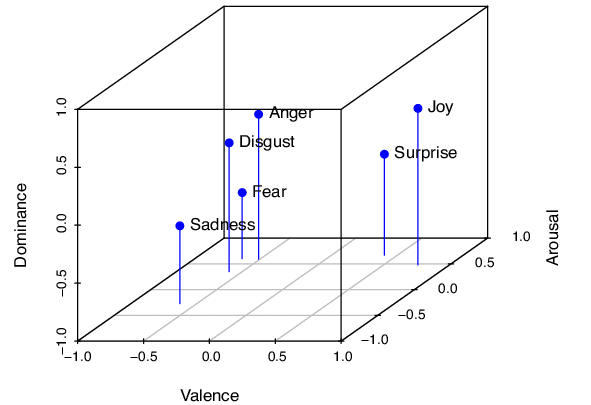
\includegraphics[width=\textwidth]{figures/3d_emotionmap.png}
      \caption{Positioning Ekman's basic emotions \cite{Ekman_Theory} on the VAD emotional space as rated by Russell and Mehrabian.\cite{VAD_model}
       Original figure taken from Buechel and Hahn's paper \cite{3d_emotions_figure}}
      \label{fig:3d_emotionmap}
    \end{minipage}
    \hfill
    \begin{minipage}[t]{0.4\textwidth}
      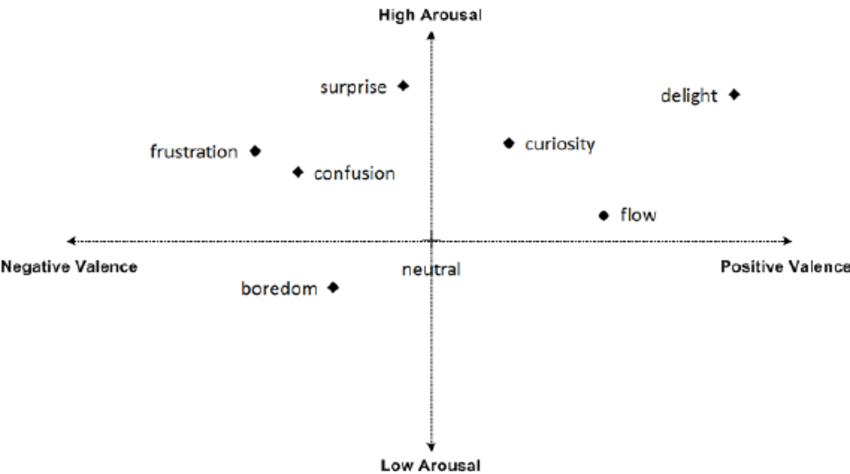
\includegraphics[width=\textwidth]{figures/2d_emotionmap.png}
      \caption{Mapping the discrete basic emotions on the valance/arousal space.
       Original figure taken from Hussain et al. paper \cite{2d_emotions_figure}}
      \label{fig:2d_emotionmap}
    \end{minipage}
  \end{figure}

\end{document}